\documentclass{article}
\usepackage{122}

\usepackage{graphicx}

\newcommand{\hr}{\par\vspace{.5\baselineskip}\noindent\hrulefill\par}

\title{Теория вероятности \\ Конспект семинара №1}

% \usepackage{xcolor}
% \pagecolor{black}
% \color{white}

\begin{document}
  \maketitle

  \hfill {\Large Веселова Юлия Александровна} \hfill

  \hfill \texttt{yul-r@mail.ru} \hfill

  $$ \Omega = \{\omega_1,\, \dots,\, \omega_n\} $$
  $$ A \subseteq \Omega \qquad P(A) = \frac{\left|A\right|}{\left|\Omega\right|} $$
  $$ C^k_n = \frac{n!}{k!(n-k)!} \qquad A^k_n = \frac{n!}{(n-k)!} $$

  \section*{№2}
  тут теоретически был номер, но он решился так быстро что я неуспел ничего записать

  \section*{№3}
  10 вариантов, 8 студентов
  $$ A = \{ \text{варианты } 1 \text{ и } 2 \text{ останутся неиспользованными} \} $$
  $$ B = \{ \text{варианты } 1 \text{ и } 2 \text{ достанутся рядом сидящим студентам} \} $$
  $$ C = \{ \text{номера распределённых вариантов можно расположить в порядке возрастания без пропусков} \} $$

  \vspace{.5cm}\noindent
  $ P(A) = \dfrac{1}{C^8_{10}} = \dfrac{1}{45} $ \hfill
  $ P(B) = \dfrac{2\cdot 7 \cdot A^6_8}{A^8_{10}} = \dfrac{14 \cdot 8!}{10!} = \dfrac{7}{45} $ \hfill
  $ P(C) = \dfrac{3}{C^8_{10}} = \dfrac{3}{45} $

  \section*{№6}
  \begin{enumerate}
    \item ЧАСЫ \\
      $ \left|\Omega\right| = n! = 4! = 24 $ \\
      $ \left|A\right| = 1 $ \\
      $ P(A) = \dfrac{1}{24} $
    \item АБРАКАДАБРА \\
      это всё эквивалентно АААААББРРДК \\
      $ \left|\Omega\right| = n! = 11! = 39916800 $ \\
      $ \left|A\right| = 5! \cdot 2! \cdot 2! $ \\
      $ P(A) = \dfrac{5! \cdot 2! \cdot 2!}{11!} = \dfrac{1}{83160} $
  \end{enumerate}

  \newpage
  \section*{№4}
  колода из 52 карт (там 4 туза); делим на две пачки
  $$ A = \{ \text{в каждой пачке по } 2 \text{ туза} \} $$
  $$ B = \{ \text{все тузы в одной пачке} \} $$
  $$ C = \{ \text{в одной пачке } 1 \text{ туз, а в другой } 3 \} $$

  \vspace{.5cm}
  $$\begin{matrix}
    \left|\Omega\right| = C^{26}_{52} \hfill \qquad &  \\[.3cm]
    \left|A\right| = C^{2}_{4} \cdot C^{24}_{48} \hfill \qquad &
      P(A) = \dfrac{C^{2}_{4} \cdot C^{24}_{48}}{C^{26}_{52}} \hfill = \dfrac{325}{833} \\[.3cm]
    \left|B\right| = C^{22}_{48} + C^{26}_{48} = 2 \cdot C^{22}_{48} \hfill \qquad &
      P(B) = \dfrac{2 \cdot C^{22}_{48}}{C^{26}_{52}} \hfill = \dfrac{92}{833} \\[.3cm]
    \left|C\right| = C^{3}_{4} \cdot \left(C^{25}_{48} + C^{23}_{48} \right) = 4 \cdot 2 \cdot C^{23}_{52} \hfill \qquad &
      P(C) = \dfrac{8 \cdot C^{23}_{52}}{C^{26}_{52}} \hfill = \dfrac{416}{833} \\[.3cm]
  \end{matrix}$$

  \section*{№8}
  из циферок 1, 2 и 3 составляется 6значное число \\
  найти вероятность того что будет одна 1ца, две 2ки и три 3ки

  \vspace{.5cm}\noindent
  у нас тут $6$ мест куда можно поставить одну 1цу и потом из оставшихся 5ти надо выбрать те 2 которые 2ки \\
  $ \left|\Omega\right| = 3^6 $ \\
  $ \left|A\right| = 6 \cdot C^2_5 $ \qquad \\
  $ P(A) = \dfrac{6 \cdot C^2_5}{3^6} = \dfrac{60}{729} = \dfrac{20}{243} $

  \hr
  \section*{Домашнее задание}
  \section*{№1}
  \begin{enumerate}[label=\realasbuk*)]
    \item $\ds P(A_k) = \f{k-1}{17}$ \qquad минус один, тк пряники мы считаем с 1 а не с 0 \\
      тут ещё надо ограничить $k$, поэтому ответ будет
      $\ds P(A_k) = \f{\min\l(k,\, 18\r)-1}{17}$
    \item $\ds P(B) = \f{2}{17} \cdot \f{1}{16} = \f{1}{136} $
    \item $\ds P(C) = \f{1}{10} \cdot \f{1}{10} = \f{1}{100} = 0.01$
  \end{enumerate}

  \section*{№5}
  количество способов $r$ человекам родится в разные дни $= A_{366}^r$,
  потомучто 29е февраля это тоже свершено нормальный день рождения.
  хотя в реальной жизни родится 29ого февраля в 4 раза сложнее, в условие написано что
  <<день рождения любого человека равновероятен в любой день года>>.
  а всего способов у $r$ человек родится $= 366^r$.
  \\ получается наша вероятность
  $\ds P(A_r) = \f{A_{366}^r}{366^r} = \f{366!}{(366-r)! \cdot 366^r}$
  \\ и для $r = 23$ будет вероятность
  $\ds P(A_{23}) = \f{366!}{(366-23)! \cdot 366^{23}} \approx 0.49\dots$

  \section*{№6 (again)}
  \begin{enumerate}[start=3]
    \item АНАНАС \\
    это всё эквивалентно АААННС \\
    $\ds \l|\Omega\r| = n! = 6! = 720 $ \\
    $\ds \l|A\r| = 3! \cdot 2! = 12 $ \\
    $\ds P(A) = \f{3! \cdot 2!}{6!} = \f{12}{720} = \f{1}{60} $
  \end{enumerate}

  \section*{№7}
  это же вроде №5 только с другими числами? \\
  $\ds P(A) = \f{30!}{(30-5)! \cdot 30^5} = \f{2639}{3750} = 0.7037\overline{3}$

  \section*{№11}
  \begin{enumerate}[label=\realasbuk*)]
    \item $\ds \f{C^6_6}{C^6_{10}} = \f{1}{C^6_{10}} = \f{1}{210}$
    \item $\ds \f{C^4_6 \cdot C^2_4}{C^6_{10}} = \f{90}{210} = \f{3}{7}$
    \item $\ds 1-\f{C^6_6}{C^6_{10}} = 1-\f{1}{C^6_{10}} = 1-\f{1}{210} = \f{209}{210}$
  \end{enumerate}

  \section*{№12}
  случаи, в которых все три числа разные, могут выпасть одним из $3! = 6$ способов,
  случаи, в которых два числа одинаковые, могут выпасть одним из $3$ способов,
  а случаи, в которых все числа разные, могут выпасть одним способом.
  получается $11$ в сумме у нас может выпасть $6+6+3+6+3+3=27$ способами,
  а $12$ -- $6+6+3+3+6+1=25$.
  парадокса больше нет. можете не благодарить.

  \section*{№13}
  это же вроде №4 только с другими числами?
  \begin{enumerate}[label=\realasbuk*)]
    \item $\ds P(A) = \f{2 \cdot C^3_{12}}{C^9_{18}} = \f{2}{221} \approx 0.009 $
    \item $\ds P(B) = \f{C^3_6 \cdot C^6_{12}}{C^9_{18}} = \f{84}{221} \approx 0.38 $
  \end{enumerate}

  \section*{№14}
  $\ds \l|\Omega\r| = C^7_{10}$ \\
  $\ds \l|A\r| = 5 \cdot 3 \cdot 2$ \\
  $\ds P(A) = \f{5 \cdot 3 \cdot 2}{C^7_{10}} = \f{30}{120} = \f{1}{4} = 0.25$

  \hr
  \section*{Условия}
  \includegraphics[page=43, width=0.3\textwidth]{./books/учебник теорвер.pdf} \hfill
  \includegraphics[page=44, width=0.3\textwidth]{./books/учебник теорвер.pdf} \hfill
  \includegraphics[page=45, width=0.3\textwidth]{./books/учебник теорвер.pdf} \hfill

  \section*{Ответы}
  \includegraphics[page=214, width=\textwidth, trim={0 10.5cm 0 2cm}, clip]{./books/учебник теорвер.pdf}
\end{document}
